\section{Analisi dei problemi}
\subsection{Tecniche di computer vision}
Per riconoscere un singolo elemento in un'immagine viene tipicamente utilizzata una Convolutional Neural Networks (CNN) allenata con grandi quantità di immagini che possono essere tranquillamente reperite in rete già raggruppate in datasets come ad esempio ImageNet.
La vera sfida salta fuori non appena ci troviamo a dover identificare nella stessa immagine diversi oggetti appartenenti a categorie diverse, di differenti dimensioni e posizioni e talvolta anche sovrapposti. Questa situazione è molto comune quando osserviamo qualsiasi foto rappresentante il mondo reale. Il risultato ottimale sarebbe quindi di avere una label di dimensioni corrette per ogni oggetto identificato mostrando anche la categoria di appartenenza dell'elemento e la probabilità che la classificazione sia effettivamente quella corretta.
\begin{figure}[H]
	\centering
	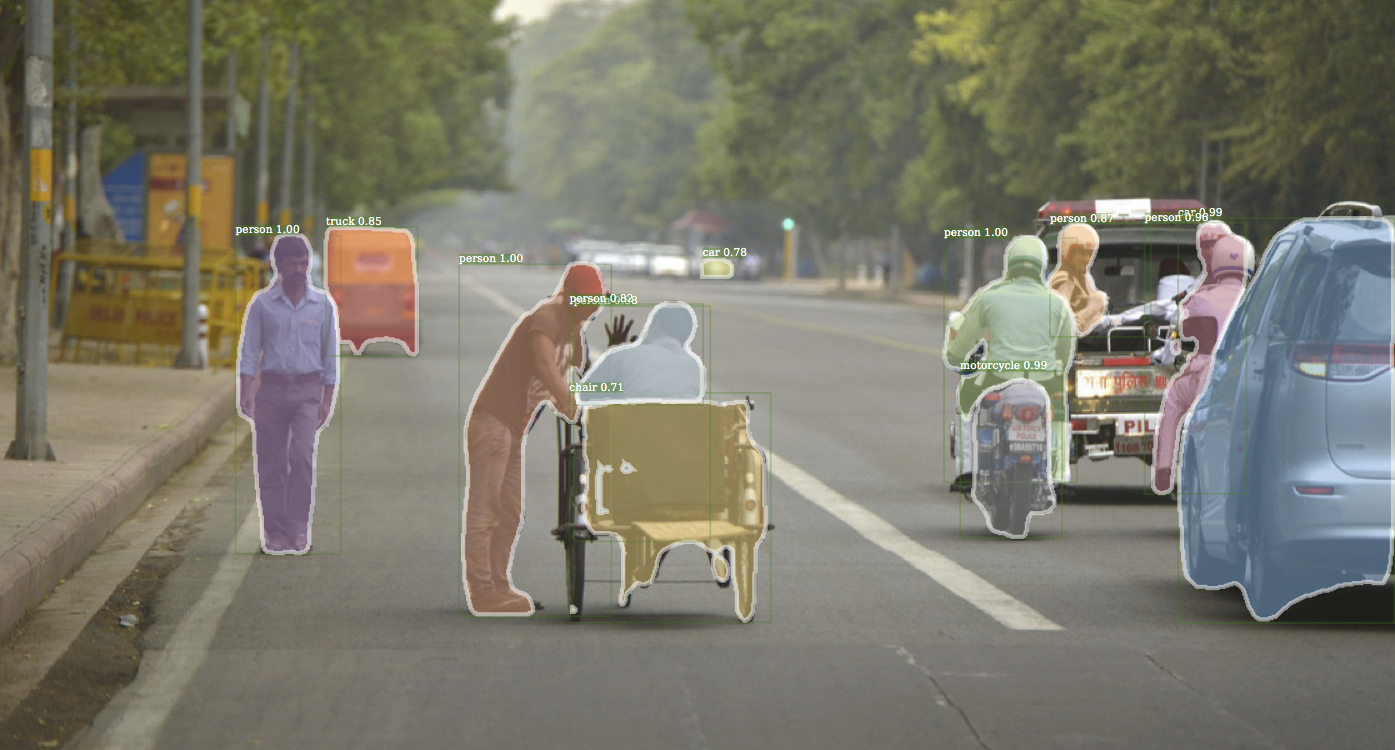
\includegraphics[width=0.7\linewidth]{images/Esempio-computer-vision.jpg}
	\caption{Esempio di un'immagine con label, categoria e probabilità per ogni elemento riconosciuto in essa}
	\label{Esempio di un frame di un video in 4K}
\end{figure}
Il modo più semplice per andare incontro a questo problema è quello di utilizzare una R-CNN (Regional Convolutional Neural Network) che tramite un algoritmo greedy chiamato Selective Search estrae delle regioni di interesse nelle quali è probabile che sia presente un oggetto. Queste regioni vengono poi date singolarmente in input ad una normale CNN la quale ha il compito di estrarne le caratteristiche principali e poi utilizzare una Support Vector Machine (SVM) presente nell'ultimo strato della CNN per rilevare la presenza di un oggetto ed eventualmente classificarlo. Questo tipo di soluzione presenta il difetto di richiedere molto tempo durante l'operazione di ricerca delle regioni di interesse.
La versione più avanzata della R-CNN ed attualmente in uso nei sistemi di computer vision attuali è chiamata Faster R-CNN e risolve il bottleneck della sua antecedente sostituendo la Selective Research con una Region Proposal Network (RPN). Con una CNN viene prima costruita la mappa delle caratteristiche più significative dell'immagine, in seguito vengono passate queste caratteristiche ad una RPN la quale ritorna delle regioni associate ad un probabilità che esse contengano un oggetto. Infine queste regioni vengono passate ad una
R-CNN che avrà come al solito il compito di riconoscere e classificare l'oggetto.
\subsection{Computer vision applicata su immagini ad alta risoluzione}
Sebbene sul web sia abbastanza facile reperire grandi quantità di immagini con cui allenare i propri modelli, però la maggior parte di questi datasets contiene solamente immagini a bassa risoluzione ed è difficile trovare in rete grandi datasets di immagini o video in 4K. Inoltre, la maggior parte dei modelli sono stati progettati per lavorare su immagini a bassa risoluzione (tra 200 e 300 pixels) sia per il fatto che una bassa risoluzione è comunque sufficiente per riconoscere e classificare un elemento, sia perchè è più efficiente lavorare su immagini di bassa qualità che su immagini in 4K.\\
Lo svantaggio che questo comporta è che nelle immagini in bassa risoluzione si perdono molti dei dettagli che invece potrebbero essere catturati da un immagine o video ad alta risoluzione. In aggiunta, i video in 4K o addirittura 8K sono sempre più diffusi al giorno d'oggi perciò anche gli attuali modelli dovranno prima o poi adattarsi per trattare efficacemente immagini di tali risoluzioni. In figura si può vedere un esempio di un frame in alta risoluzione, diminuendone le dimensioni, perdendo quindi qualità, non sarebbe stato possibile riconoscere alcune delle persone individuate nel frame.
\begin{figure}[H]
	\centering
	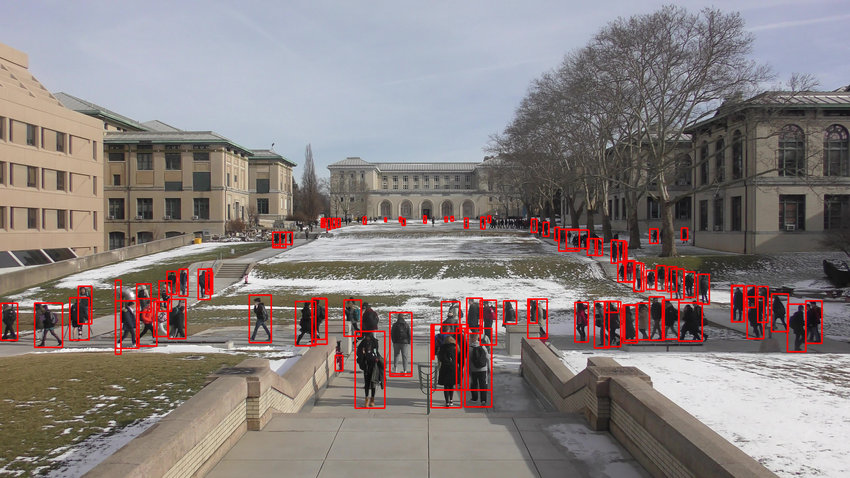
\includegraphics[width=0.7\linewidth]{images/Esempio-4K-video-frame.png}
	\caption{Esempio di un frame di un video in 4K}
	\label{Esempio di un frame di un video in 4K}
\end{figure}
\subsection{Frammentazione dell'immagine}
Un'immagine in 4K ha una risoluzione di 3840 x 2160 pixels con un totale di 8294400 di pixels. Una rete neurale in grado di ricevere un input così corposo dovrebbe allenare un numero molto elevato di parametri risultando così in un processo molto lungo e dispendioso. L'idea è quella di frammentare l'immagine in diverse sotto-immagini di dimensioni minori e quindi gestibili efficacemente da una singola rete neurale.
(FIGURA)
Tuttavia questo procedimento non è esente da difficoltà,  nel caso in cui un oggetto dovesse trovarsi su più regioni diverse esso potrebbe venire identificato più volte ed essere riconosciuto ogni volta come se fosse un oggetto diverso.\\
Un primo approccio per risolvere questo problema è stato quello di porre maggiore attenzione alle labels degli oggetti posizionate in prossimità dei confini delle regioni in quanto con molta probabilità è possibile che l'oggetto continui invece nella regione adiacente. Se quindi presente una label anche nella regione adiacente allora si è passati al controllo che le labels possano effettivamente appartenere allo stesso elemento. Per fare ciò è stato sufficiente assicurarsi che le due labels combaciassero entro una certa soglia ed in caso affermativo fonderle in una sola label che contenesse l'oggetto intero.\\
Un' altra soluzione esaminata è stata quella di suddividere l'immagine intera in regioni con sovrapposizione. In questo modo un elemento giacente a ridosso tra una o più regioni avrebbe generato due o più labels sovrapposte. Tramite un algoritmo di Non-Maximum Suppression, per ogni insieme di labels parzialmente sovrapposte, sono state eliminate le labels con probabilità minore tenendo valida solo quella con probabilità massima.